% generado por el cuaderno homónimo; no editar
\begin{subfigure}[t]{0.49\textwidth}
    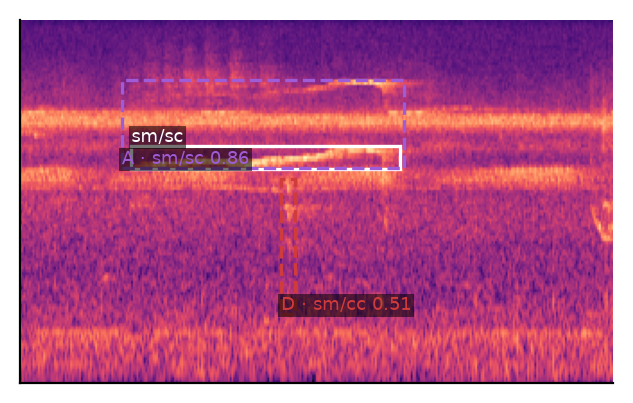
\includegraphics[width=\linewidth]{figures/RE_3-3/ejemplo_1}
    \caption{A encuadre: \code{20240411\_104931.wav}, ventana 1100}
\end{subfigure}\hfill
\begin{subfigure}[t]{0.49\textwidth}
    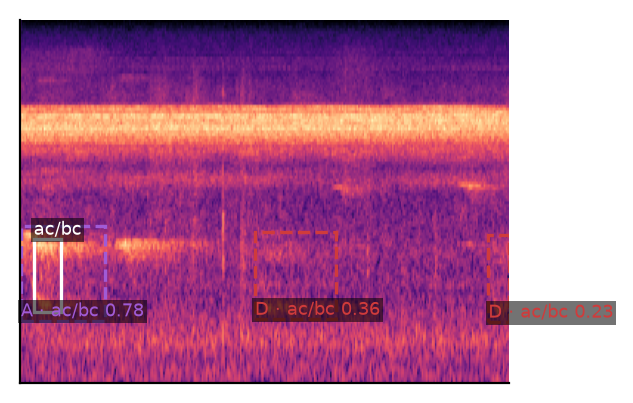
\includegraphics[width=\linewidth]{figures/RE_3-3/ejemplo_2}
    \caption{A encuadre: \code{20240617\_152116.wav}, ventana 6312}
\end{subfigure}\\[1.5ex]
\begin{subfigure}[t]{0.49\textwidth}
    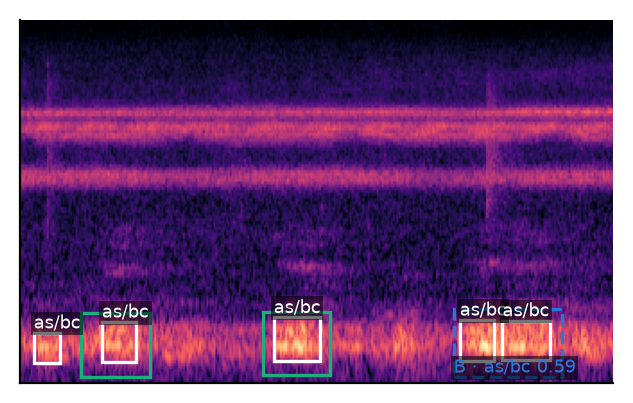
\includegraphics[width=\linewidth]{figures/RE_3-3/ejemplo_3}
    \caption{B unidad: \code{20240523\_120404.wav}, ventana 3955}
\end{subfigure}\hfill
\begin{subfigure}[t]{0.49\textwidth}
    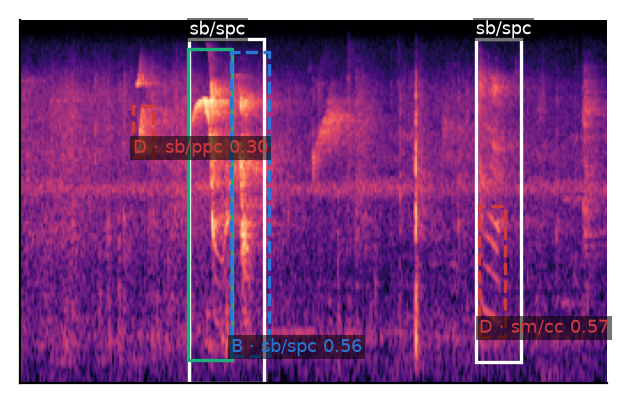
\includegraphics[width=\linewidth]{figures/RE_3-3/ejemplo_4}
    \caption{B unidad: \code{20240516\_083217.wav}, ventana 2242}
\end{subfigure}\\[1.5ex]
\begin{subfigure}[t]{0.49\textwidth}
    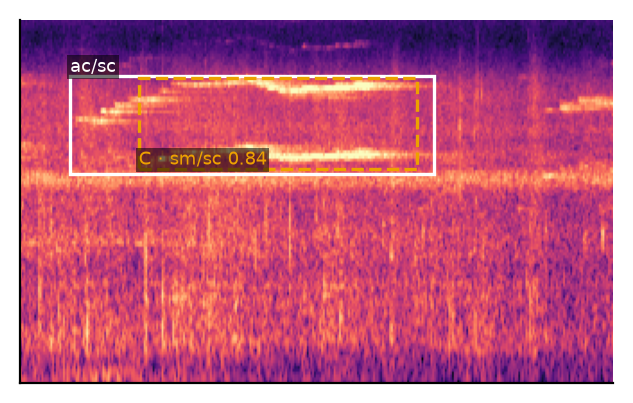
\includegraphics[width=\linewidth]{figures/RE_3-3/ejemplo_5}
    \caption{C clase: \code{20240227\_085004.wav}, ventana 784}
\end{subfigure}\hfill
\begin{subfigure}[t]{0.49\textwidth}
    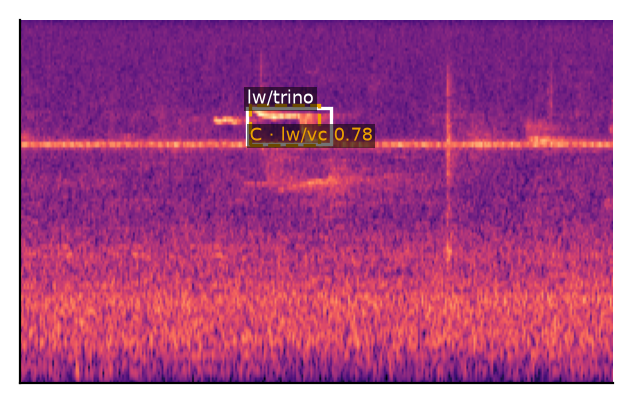
\includegraphics[width=\linewidth]{figures/RE_3-3/ejemplo_6}
    \caption{C clase: \code{20240520\_070831.wav}, ventana 2560}
\end{subfigure}\\[1.5ex]
\begin{subfigure}[t]{0.49\textwidth}
    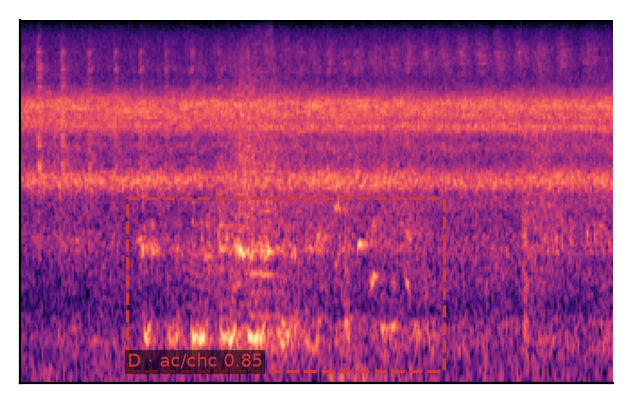
\includegraphics[width=\linewidth]{figures/RE_3-3/ejemplo_7}
    \caption{D sin anotación: \code{20240227\_090548.wav}, ventana 824}
\end{subfigure}\hfill
\begin{subfigure}[t]{0.49\textwidth}
    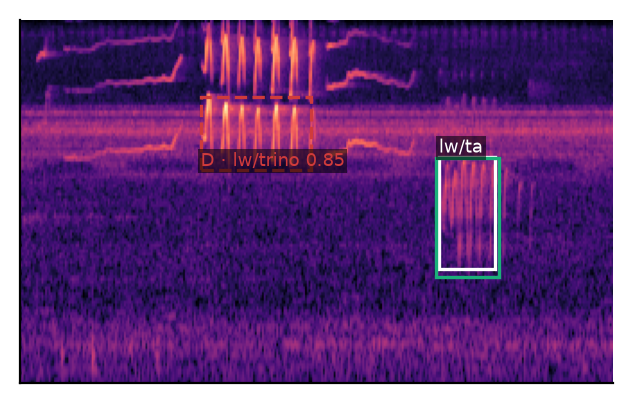
\includegraphics[width=\linewidth]{figures/RE_3-3/ejemplo_8}
    \caption{D sin anotación: \code{20240125\_162433.wav}, ventana 2127}
\end{subfigure}
